
Further injection tests in real data.

%\subsection{Real S6 data: p-weighted $h_0$ recovered vs injected at 142 Hz}
%\begin{figure}
%\caption{\protect\includegraphics[width=0.4\paperwidth,height=0.2\paperheight]{plots/p-weighted/h0UL-vs-h0injected-162-0Hz.eps}}
%Raw $h_0$, and tentative 95\% confidence UL, for 500 injections into\\
%S6 data at 142 Hz (injections also done at 162, 222 Hz)
%\end{figure}

\subsection{Real S6 data: detection efficiency at 162 Hz}

\begin{figure}
\begin{center}
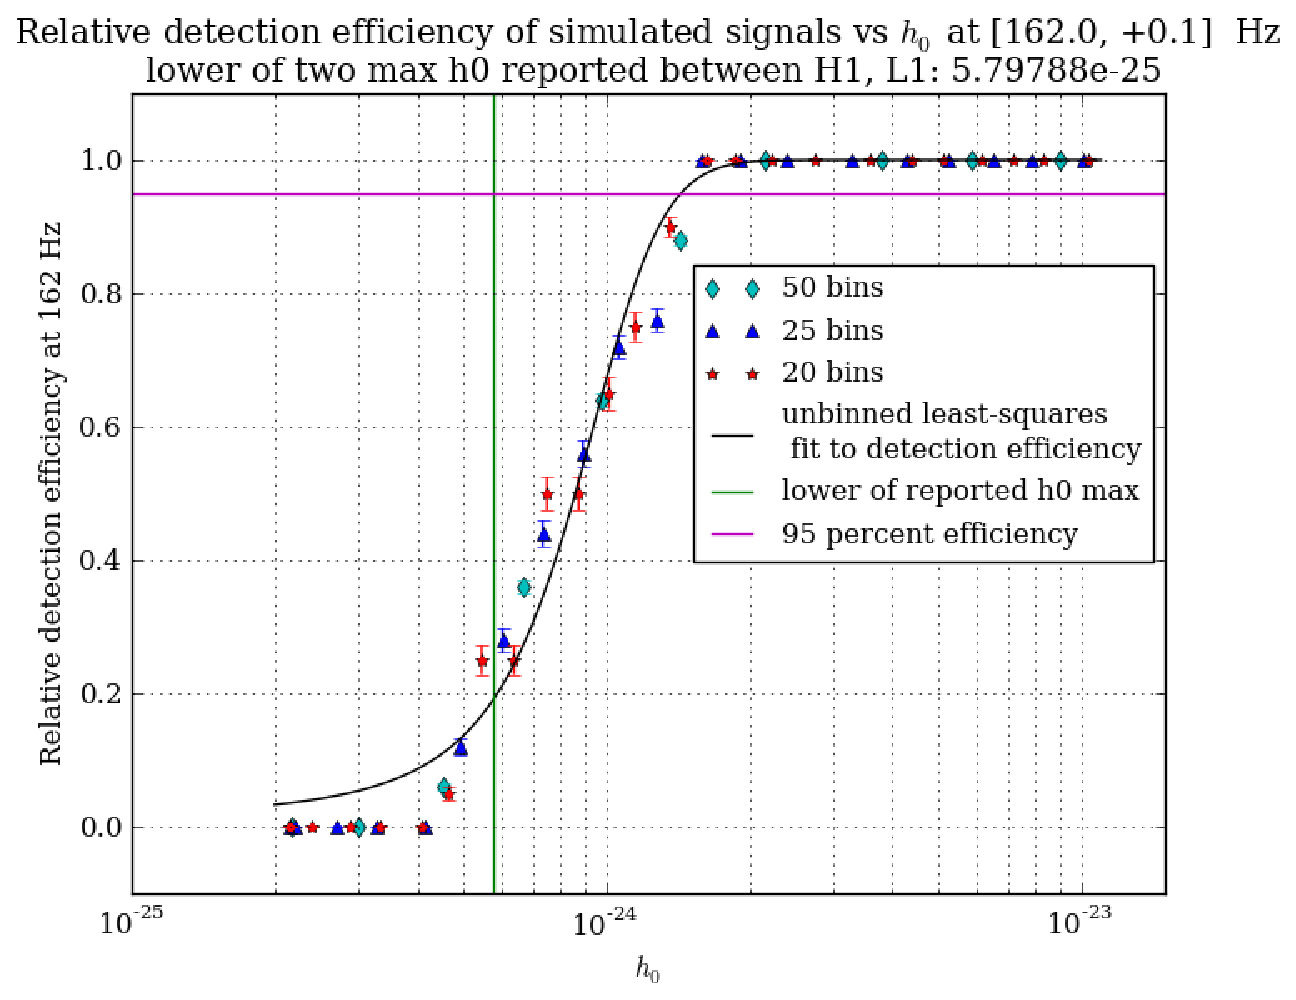
\includegraphics[width=0.4\paperwidth,height=0.2\paperheight]{plots/detectionEfficiencyh0-162-0Hz.eps}
\caption{
Detection efficiency of 500 injections (each at H1, L1) into
S6 data at 162 Hz, given threshold log10p = -7.75}
\end{center}
\end{figure}

\subsubsection{Real S6 data: $h_0$ recovered vs injected}

\begin{figure}
\begin{center}
\includegraphics[width=0.4\paperwidth,height=0.2\paperheight]{plots/h0UL-vs-h0injected-162-0Hz.eps}
\caption{
Raw $h_0$ \& tentative 95\% confidence UL $>2\times10^{-24}$; 500 injections
into S6 data at 162 Hz (injections also done at 142, 222 Hz)}
\end{center}
\end{figure}

%\subsubsection{Real S6 data: $p$-weighted $h_0$ recovered vs injected}
%\begin{figure}
%\caption{\protect\includegraphics[width=0.4\paperwidth,height=0.2\paperheight]{plots/p-weighted/h0UL-vs-h0injected-162-0Hz.eps}}
%Raw $h_0$, and tentative 95\% confidence UL, for 500 injections into\\
%S6 data at 162 Hz (injections also done at 142, 222 Hz)
%\end{figure}



\subsection{Real data: detection efficiency at 222 Hz}

\begin{figure}
\begin{center}
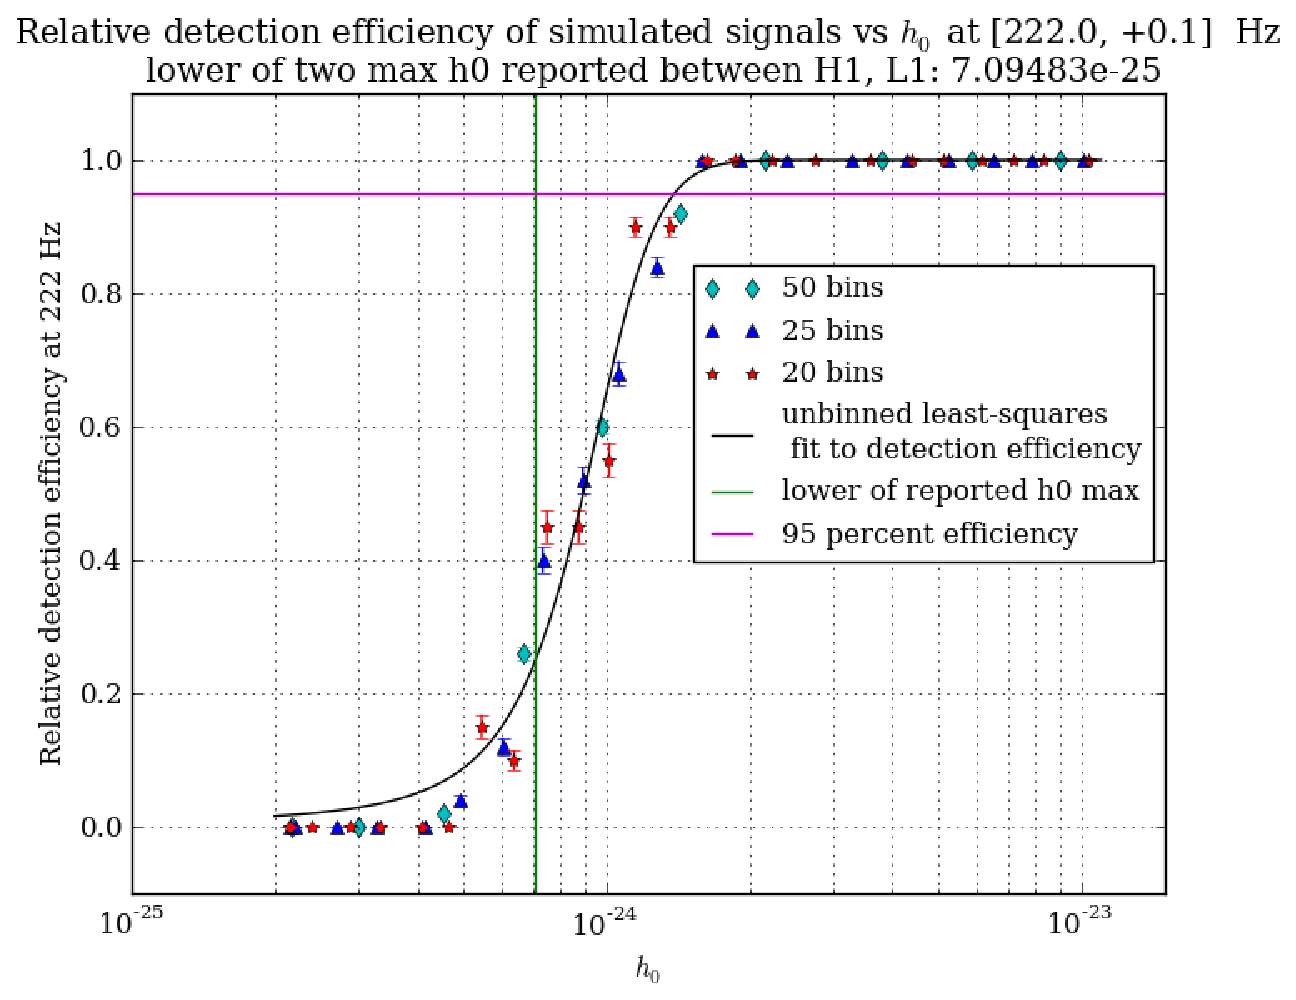
\includegraphics[width=0.4\paperwidth,height=0.2\paperheight]{plots/detectionEfficiencyh0-222-0Hz.eps}
\caption{
Detection efficiency of 500 injections (each at H1, L1) into
S6 data at 222 Hz, given threshold log10p = -7.75}
\end{center}
\end{figure}

\subsubsection{Real S6 data: $h_0$ recovered vs injected}

\begin{figure}
\begin{center}
\includegraphics[width=0.4\paperwidth,height=0.2\paperheight]{plots/h0UL-vs-h0injected-222-0Hz.eps}
\caption{
Raw $h_0$ \& tentative 95\% confidence UL $>2\times10^{-24}$; 500 injections
into S6 data at 222 Hz (injections also done at 142, 162 Hz)}
\end{center}
\end{figure}

%\subsubsection{Real S6 data: $p$-weighted $h_0$ recovered vs injected}
%\begin{figure}
%\caption{\protect\includegraphics[width=0.4\paperwidth,height=0.2\paperheight]{plots/p-weighted/h0UL-vs-h0injected-222-0Hz.eps}}
%Raw $h_0$, and tentative 95\% confidence UL, for 500 injections into\\
%S6 data at 222 Hz (injections also done at 142, 162 Hz)
%\end{figure}


%\subsection{S6: $p$-weighted Sco X-1 upper limits, random polarization}
%\begin{figure}
%\caption{\protect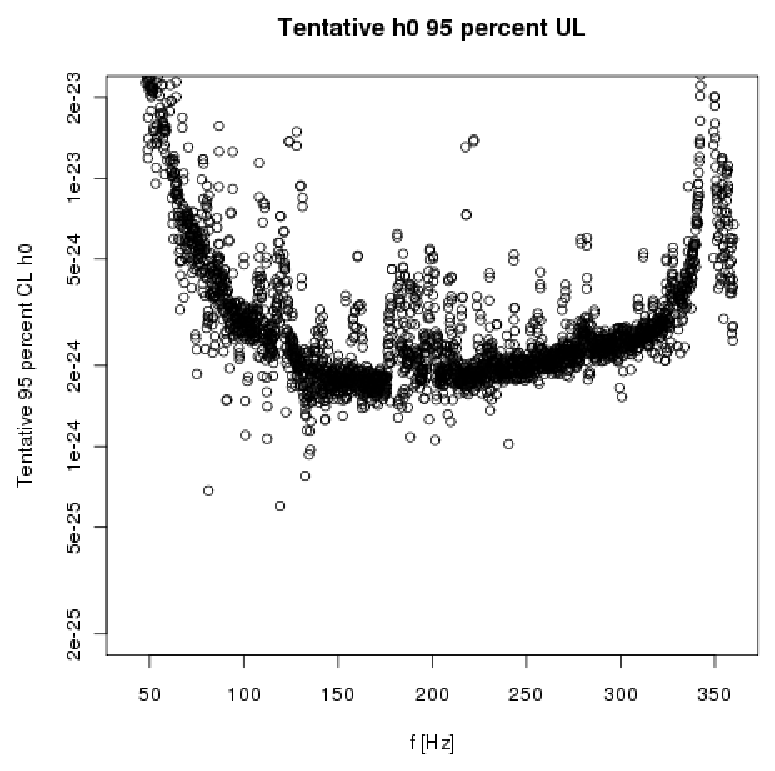
\includegraphics[width=0.4\paperwidth,height=0.2\paperheight]{plots/p-weighted/h0FullUL95logGuess-H1.eps}}
%H1: loudest $h_0 \times \left( 1 + \frac{\log_{10} p}{-7.75} \right) \times \left[\cos \iota \textup{ factor}\right]$ in 0.1 Hz bands
%\end{figure}
%\begin{figure}
%\caption{\protect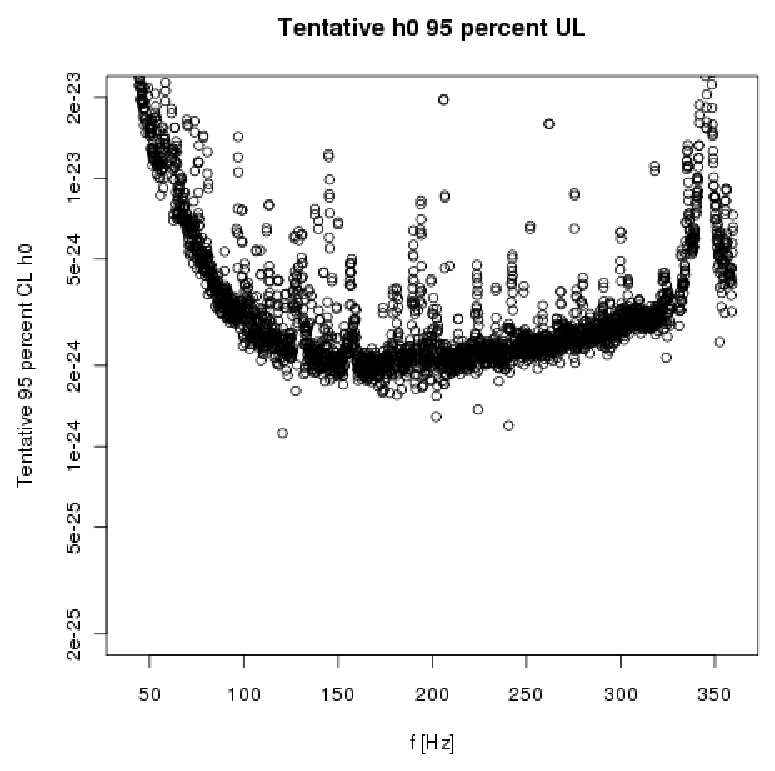
\includegraphics[width=0.4\paperwidth,height=0.2\paperheight]{plots/p-weighted/h0FullUL95logGuess-L1.eps}}
%L1: loudest $h_0 \times \left( 1 + \frac{\log_{10} p}{-7.75} \right) \times \left[\cos \iota \textup{ factor}\right]$ in 0.1 Hz bands
%\end{figure}

\subsection{S6: Scorpius X-1 upper limits, raw circular output}

\begin{figure}
\begin{center}
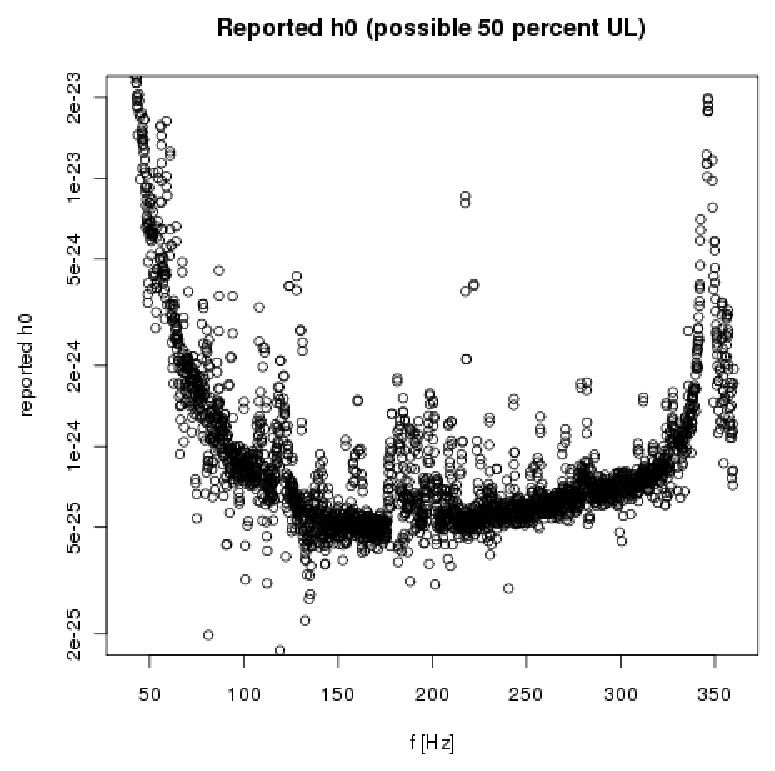
\includegraphics[width=0.4\paperwidth,height=0.2\paperheight]{plots/h0FullUL50log-H1.eps}
\caption{
H1: loudest $h_0$ in 0.1 Hz bands, effectively circular polarization}
\end{center}
\end{figure}

\begin{figure}
\begin{center}
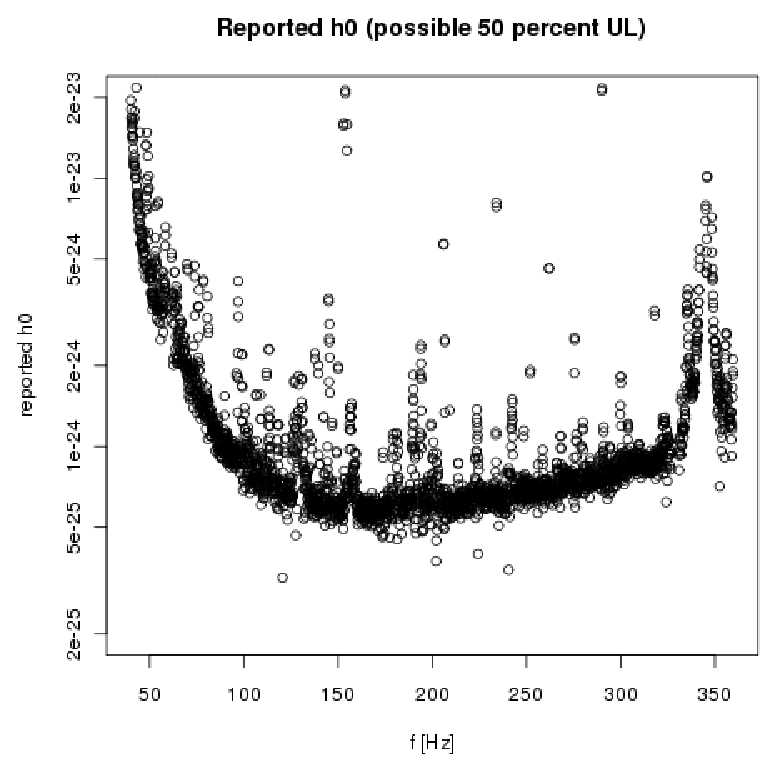
\includegraphics[width=0.4\paperwidth,height=0.2\paperheight]{plots/h0FullUL50log-L1.eps}
\caption{
L1: loudest $h_0$ in 0.1 Hz bands, effectively circular polarization}
\end{center}
\end{figure}
